\chapter{Testovací program}
Testovací systém běžící na serveru testovací laboratoře se skládá z několika samostaných částí. Základem celého systému je databáze uchovávající všechna informace struktuře testovací laboratoře, informace o všech modelech testovaných zařízení, data s výsledky jednotlivých testů. Program testlab jenž se stará o celý průběh testování. Několika málo přepínači lze nastavit průběh testování. Další součástí je sada programů nazývající se testovací API. Tyto programu usnadňují psaní jednotlivých testů. Nedílnou součástí testovacího systému jsou testovací skripty, které lze rozdělit na skripty pro stáhnutí projektu, kompilaci projektu, testování výrobku a úklid projektu. Tyto testovací skripty odpovídají testovacím procedurám testování založeného na modelech. Poslední součástí testovacího systému je webový interface pro sledování výsledků testování a nastavování chování testovacího systému.

\section{Adresářová struktura testovacího systému}

Jednotlivé částí testovacího systému jsou rozloženy v adresářové struktuře serveru následovně. Všechny součásti testovacího programu testlab a testovací API jsou umístěny v adresáři /usr/bin, aby byly odevšad spustitelné. Sdílené knihovny, které využívá testovací program a mohou ho využívat nové programy testovacího API jsou umístěny v adresáři /usr/lib. Hlavičkové soubory pro tyto knihovny jsou k naleznutí v adresáři /usr/include/testlab. Tato část testovacího systému se za běhu nemění a zůstává stejná. Jednou vyjímkou je aktualizace testovacího systému, při které mohou být opraveny chyby testovacího systému, či přidán nový program do testovacího API. Tuto aktualizaci provádí pouze administrátor testovacího systému.

Druhá část adresářové struktury testovacího systému obsahuje soubory a adresáře měnící se v průběhu běhu testovacího systému. Tato část se nechází v adresáři /var/testlab a je rozdělena na následující podadresáře. Adresář clean obsahuje skripty pro zajištění úklidu po překladu jednotlivých platforem. Adresář compile obsahuje skripty zajišťující kompilaci jednotlivých výrobků všech platforem. Pro každou platformu je v tomto adresáři jeden skript a výrobek se zadává jako parametr. V adresáři checkout nalezneme skripty pro stáhnutí zdrojových kódu každé platformy. Pro stahování zdrojových kódů se budou často využívat repozitáře a v systému bude konkrétně využit verzovací systém git. Project je pracovním adresářem kam jsou stahované zdrojové kódy jednotlivých platforem a kde jsou následně překládány. Dále je tento adresář rozdělen do jednotlivých podadresářů podle jednotlivých releasů překládaného firmwaru. V každém adresářy releasu jsou adresáře pro každou testovanou platformu. Adresáře jednotlivých releasu se před ukončením programu testlab mažou, jelikož dále nejsou potřeba a zabírají velký prostor na disku. Přeložený firmware všech výrobků je ukládán do adresáře firmware a do podadresáře s názevem identifikačního čísla releasu, pro který byl firmware přeložen. Firmwary se zde uchovávají většinou do vydání další verze ostrého firmwaru. Předchozí firmwary jsou zálohovány na jiný server či jiný disk testovacího serveru, pro zachování místa na systémovém ssd disku testovacího serveru. Testovací skripty se nacházejí v adresáři tests. Adresář tests se dále dělí na podadresáře s názvy testovaných funkcí, ve kterých se nacházejí jednotlivé testovací skripty jejichž název je schodný s testovací procedurou. Konfigurace nahrávané do routeru během testování jsou uloženy v adresáři conf. Adresář conf je dále rozdělen podle testovaných funkcí. V každém adresáři dané funkce jsou adresáře pojmenované podle identifikačních čísel jednotlivých routerů ve kterých se již nacházejí jednotlivé konfigurace routerů. Posledním adresářem této části testovacího systému je adresář logs. V adresáři logs se ukládají logy z jednotlivých fází testování. Ukládájí se zde logy ze stáhování zdrojových kódů, ze samotné kompilace všech výrobků a z úklidu po překladu. Adresář je členěn podle typu logu a dále podle releasu testovaného firmwaru. Logy starších releasu se stejně jako firmware přesouvají na jiný disk nebo jsou mazány. Logy ze samotných testů se jako jediné ukládají do databáze.

\begin{figure}[h]
  \centering
  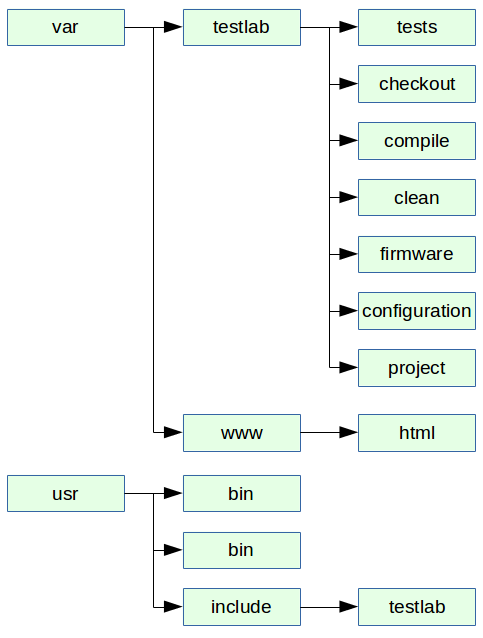
\includegraphics[width=.4\LW]{adresar_struktura}
  \caption{Adresářová struktura testovacího systému}
  \label{fig:adresar_struktura}
\end{figure}

Třetí část testovacího systému se nachází v adresáři /var/www/html. Tuto část testovacího systému tvoří samotné webové stránky testovacího systému

\section{Struktura databáze}
Jak již bylo dříve zmíněno všechny informace o testovaných zařízeních a výsldedcích testů jsou uloženy v databázi. K těmto účelům byla využita MySQL databáze. K databázi má přístup samotný testovací program testlab, všechny programy testovacího api a hlavně webová aplikace sloužící k adminitraci modelů testovaných zařízení a reportování výsledků testů. Pro organizované uchovávání všech dat byla navržena základní struktura databáze, která se časem s přibývající funkcionalitou testovacího zařízení může měnit. Jednotlivé tabulky této struktury jsou popsány v samostatných sekcích.

\subsection{Tabulka fwrelease}
První a základní tabulkou celého systému je fwreleases. V tabulce fwreleases jsou uloženy informace o testovaném releasu. Release je vytvořen a uložen do databáze při každém spuštění testování, aby bylo možné rozlišit různé testy. Všechny tabulky, které uchovávají informace o konkrétním testu odkazují právě na tuto tabulku. Tabulka fwreleases obsahuje pouze 3 údaje. Položka idfwreleases je primárním klíčem tabulky, položka date uchovává datum a čas vzniknu releasu a položka type určije o jaký typ vydání firmwaru se jedná.

\begin{figure}[h]
  \centering
  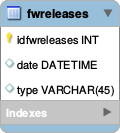
\includegraphics[scale=0.8]{database_fwreleases}
  \caption{Tabulka fwreleases}
  \label{fig:database_fwreleases}
\end{figure}

\subsection{Tabulka platforms}
Tabulka platforms obsahuje informace o jednotlivých platformách. Platforma je skupina výrobků postavena na společných zdrojových kódech a na jednom procesoru. Platformy se dále dělí na výrobky. Tabulka obsahuje prozatím následující 4 položky. Položka idplatforms, která je primárním klíčem tabulky, položka name slouží k uložení názvu tabulky, dále položky timeout\_checkout a timeout\_build sloužící k nastavení timeoutu skriptu pro stažení zdrojových kódu platfromy a pro přeložení zfrojových kódů platformy.

\begin{figure}[h]
  \centering
  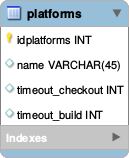
\includegraphics[scale=0.8]{database_platforms}
  \caption{Tabulka platforms}
  \label{fig:database_platforms}
\end{figure}

\subsection{Tabulka products}
Tabulka products obsahuje informace o jednotlivých produktech. V této tabulce nejsou produkty chápány jako jednotlivé produkty v testovací laboratoři, ale pouze jednotlivé druhy firmwaru. Rozdělení bylo provedeno z důvodu možnosti nahrání stejného firmwaru do různého hardwaru a tímto vznikne nový výrobek. Tabulka products obsahuje pouze 3 následující položky. Položka idproducts, které je primárním klíčem tabulky, položka idplatforms odkazující na danou platformu v tabulce platforms. Poslední položka name definuje název produktu.

\begin{figure}[h]
  \centering
  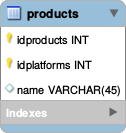
\includegraphics[scale=0.8]{database_products}
  \caption{Tabulka products}
  \label{fig:database_products}
\end{figure}

\subsection{Tabulka checkout}
Tabulka checkout slouží pro ukládání výsledků ze stažení zdrojových kódů z repozitáře. Tabulka obsahuje 4 položky. Položka idcheckout je primárním klíčem tabulky. Položka idplatforms odkazuje na tabulku platforms a udává o jaké zdrojové kódy platformy se jedná. Položka idfwreleases odkazuje na tabulku fwreleases a udává k jakému testování výsledek odpovídá. Poslední položka state ukládá stav výsledku skriptu pro stažení aktuálních zdrojových kódů platformy.

\begin{figure}[h]
  \centering
  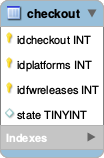
\includegraphics[scale=0.8]{database_checkout}
  \caption{Tabulka checkout}
  \label{fig:database_checkout}
\end{figure}

\subsection{Tabulka builds platform}
Tabulka builds\_platform slouží pro ukládání výsledků překladu celé platformy, čili všech výrobků dané platformy. Tabulka obsahuje celkem 4 položky. Položka idbuilds\_platform je primárním klíčem tabulky. Položka idplatforms odkazuje na tabulku platforms a udává jaké platformy se výsledek překladu týká. Položka idfwreleases odkazuje na tabulku fwreleases a udává k jakému vydání firmwaru je zdrojový kód překládán. Poslední položka state představuje stav ukončení překladu firmwaru pro celou platformu.

\begin{figure}[h]
  \centering
  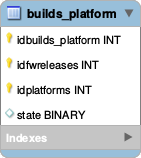
\includegraphics[scale=0.8]{database_buildsplatform}
  \caption{Tabulka builds platform}
  \label{fig:database_buildsplatform}
\end{figure}

\subsection{Tabulka build product}
Tabulka builds\_product slouží pro ukládání výsledků překladu jednotlivých výrobků. Tabulka obsahuje celkem 4 položky. Položka idbuilds\_product je primárním klíčem tabulky. Položka idproducts odkazuje na tabulku products a udává jakého produktu se výsledek překladu týká. Položka idfwreleases odkazuje na tabulku fwreleases a udává k jakému vydání firmwaru je zdrojový kód překládán. Poslední položka state představuje stav ukončení překladu firmwaru daného produktu.

\begin{figure}[h]
  \centering
  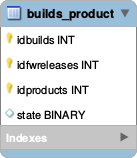
\includegraphics[scale=0.8]{database_buildsproduct}
  \caption{Tabulka builds product}
  \label{fig:database_buildsproduct}
\end{figure}

\subsection{Tabulka routers}

\begin{figure}[h]
  \centering
  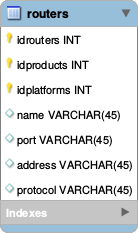
\includegraphics[scale=0.8]{database_routers}
  \caption{Tabulka routers}
  \label{fig:database_routers}
\end{figure}

\subsection{Tabulka functions}

\begin{figure}[h]
  \centering
  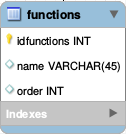
\includegraphics[scale=0.8]{database_functions}
  \caption{Tabulka functions}
  \label{fig:database_functions}
\end{figure}

\subsection{Tabulka dependences}

\begin{figure}[h]
  \centering
  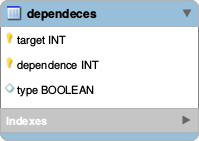
\includegraphics[scale=0.8]{database_dependences}
  \caption{Tabulka dependences}
  \label{fig:database_dependences}
\end{figure}

\subsection{Tabulka procedures}

\begin{figure}[h]
  \centering
  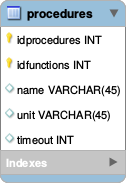
\includegraphics[scale=0.8]{database_procedures}
  \caption{Tabulka procedures}
  \label{fig:database_procedures}
\end{figure}

\subsection{Tabulka routers has functions}

\begin{figure}[h]
  \centering
  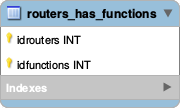
\includegraphics[scale=0.8]{databse_routershasfunctions}
  \caption{Tabulka routers has functions}
  \label{fig:databse_routershasfunctions}
\end{figure}

\subsection{Tabulka tests router}

\begin{figure}[h]
  \centering
  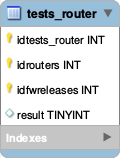
\includegraphics[scale=0.8]{database_testsrouter}
  \caption{Tabulka tests router}
  \label{fig:database_testsrouter}
\end{figure}

\subsection{Tabulka tests function}

\begin{figure}[h]
  \centering
  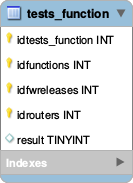
\includegraphics[scale=0.8]{database_testsfunction}
  \caption{Tabulka tests function}
  \label{fig:database_testsfunction}
\end{figure}

\subsection{Tabulka tests procedure}

\begin{figure}[h]
  \centering
  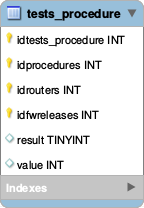
\includegraphics[scale=0.8]{database_testsprocedure}
  \caption{Tabulka tests procedure}
  \label{fig:database_testsprocedure}
\end{figure}

\subsection{Tabulka logs}

\begin{figure}[h]
  \centering
  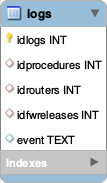
\includegraphics[scale=0.8]{database_logs}
  \caption{Tabulka logs}
  \label{fig:database_logs}
\end{figure}

\section{Popis programu}

O průběh celého testu se stará program testlab. Testlab je program psaný v jazyc C. Program po spuštění otevře systémový log pro možnost logování chyb do systémového logu. Filtrováný systémový log by měl později být zobrazován na webowém rozhraní testovacího systému. První hláškou do systémového logu je informace o spuštění programu testlab, daným uživatelem a v určený čas. Po otevření systémového logu program rozebírá parametry na příkazové řádce. Parametry jsou rozebíráný pomocí funkce getopts. Pomocí parametrů lze ovlivnit chování programu testlab !!!!!DOPLNIT PARAMETRY!!!!!!

\begin{figure}[h]
  \centering
  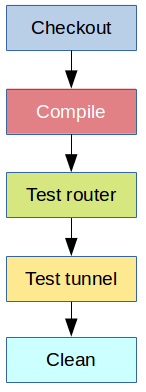
\includegraphics[width=.2\LW]{program_schema}
  \caption{Základní schéma testovacího programu}
  \label{fig:program_schema}
\end{figure}


Nyní se provádějí přípravné kroky pro samotné testování. Nejdříve je vytvořen nový release firmwaru a následně vložen do databáze. V projektovém adresáři je vytvořen nový adresář se stejným názvem jako identifikační číslo testovaného releasu.

\subsection{Checkout}
\subsection{Compile}
\subsection{Test router}
\subsection{Test tunel}
\subsection{Clean}
\subsection{Remote server}
\subsubsection{Telnet}
\subsubsection{SSH}

\endinput
